\section{Inverted Index Evaluation}
\label{sec:index}

Three structures answer the same queries over the same corpus: a JSON file,
a folder of per-term files, and a MongoDB collection. Before their numbers
are interpreted, \cref{sec:equivalence-structures} showed that they answer
identically.

\subsection{Build scalability: elapsed time and memory growth}
\label{sec:index-scalability}

Each structure is built from batches of \fixed{25} to \fixed{10{,}000} books
(\cref{tab:workload}); every batch size is repeated and the mean is plotted.
Two series are shown (\cref{fig:scalability-elapsed,fig:scalability-memory}).

\begin{figure}[htbp]
    \centering
    \begin{minipage}[t]{0.48\textwidth}
        \centering
        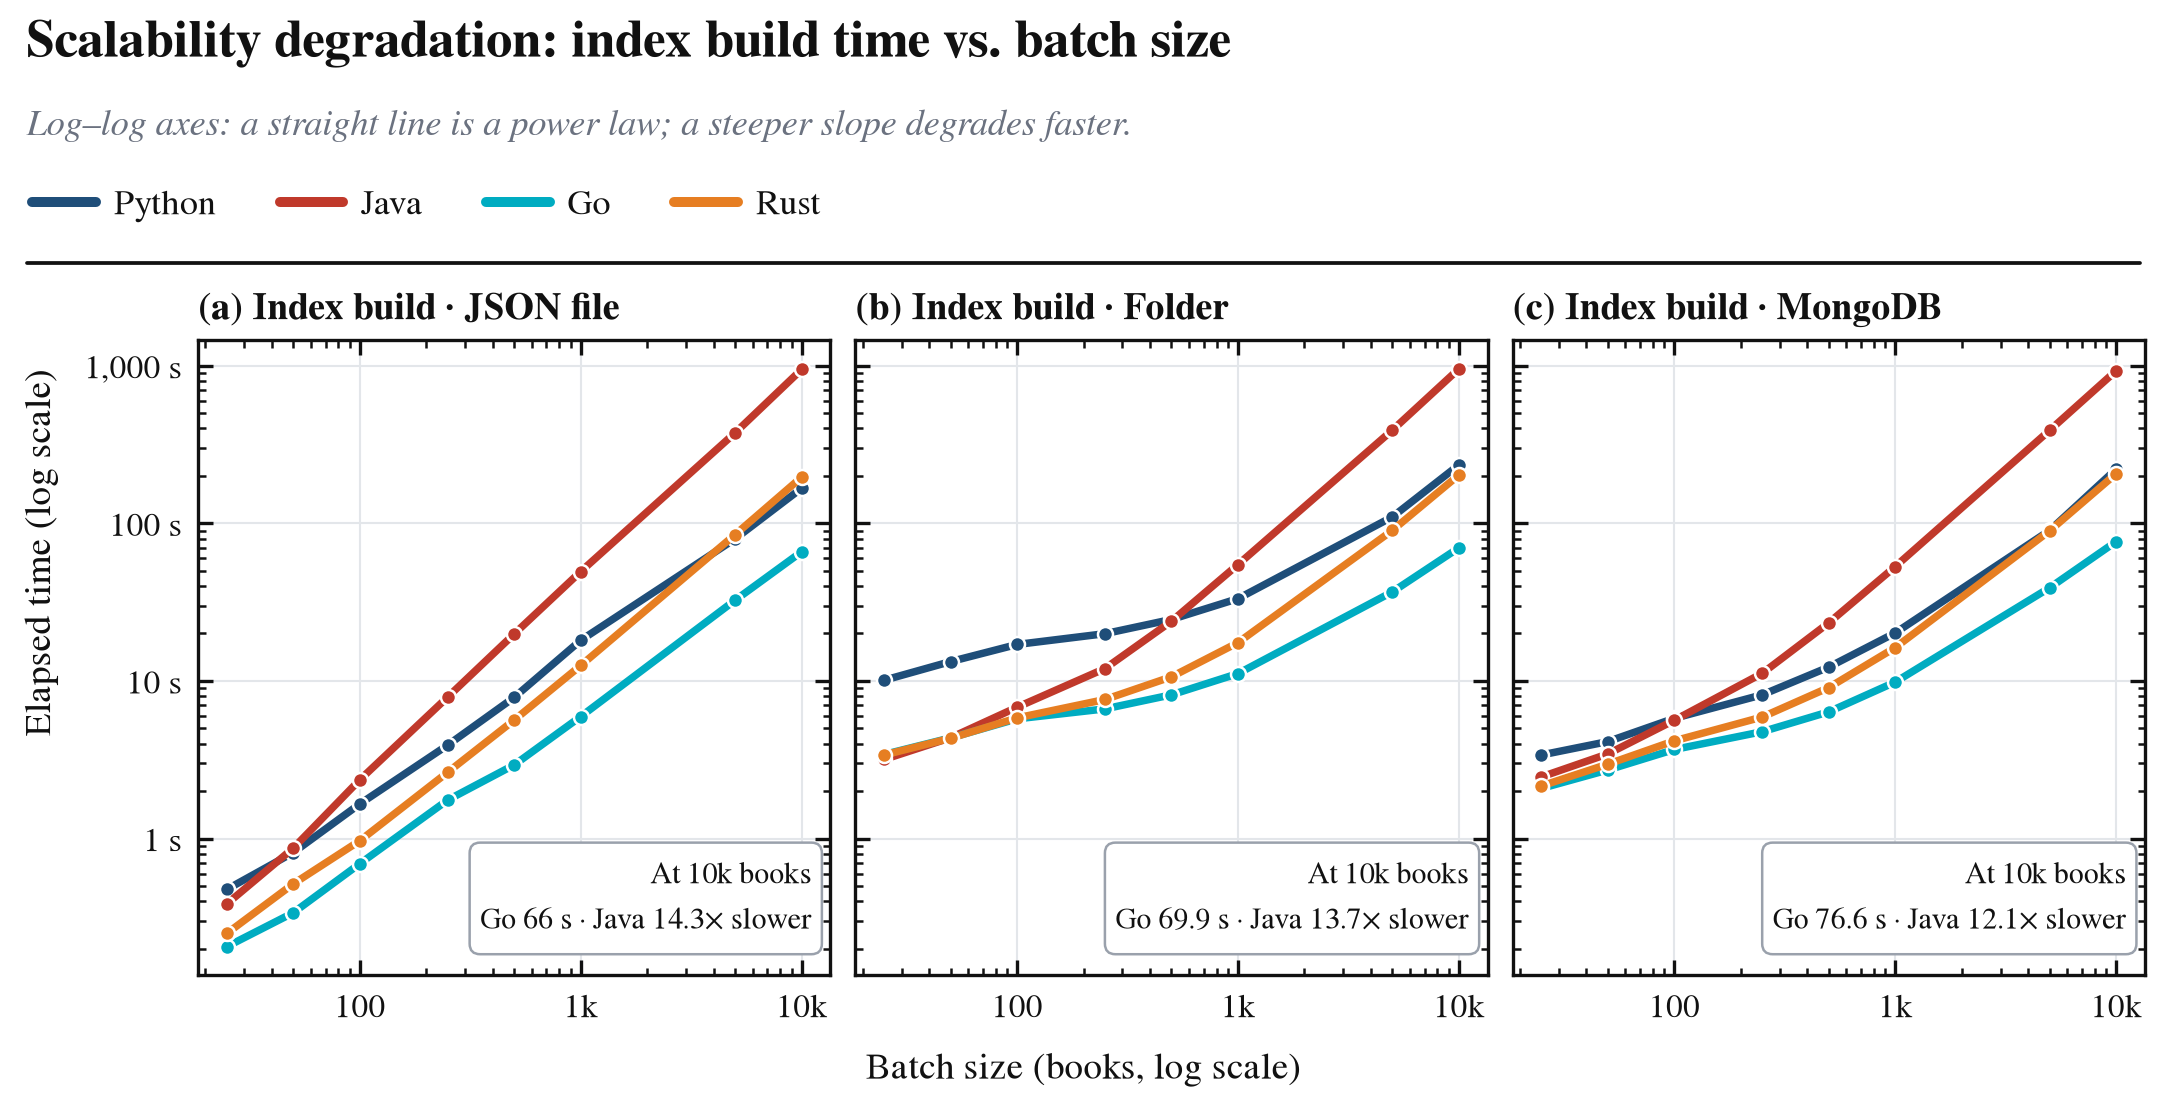
\includegraphics[width=0.94\textwidth]{scalability/scalability_elapsed.png}
        \caption{Build elapsed time versus batch size (log--log), mean of
        5 repetitions up to 1{,}000 books, 3 at 5{,}000 and 2 at 10{,}000
        (\texttt{scalability.csv}).}
        \label{fig:scalability-elapsed}
    \end{minipage}\hfill
    \begin{minipage}[t]{0.48\textwidth}
        \centering
        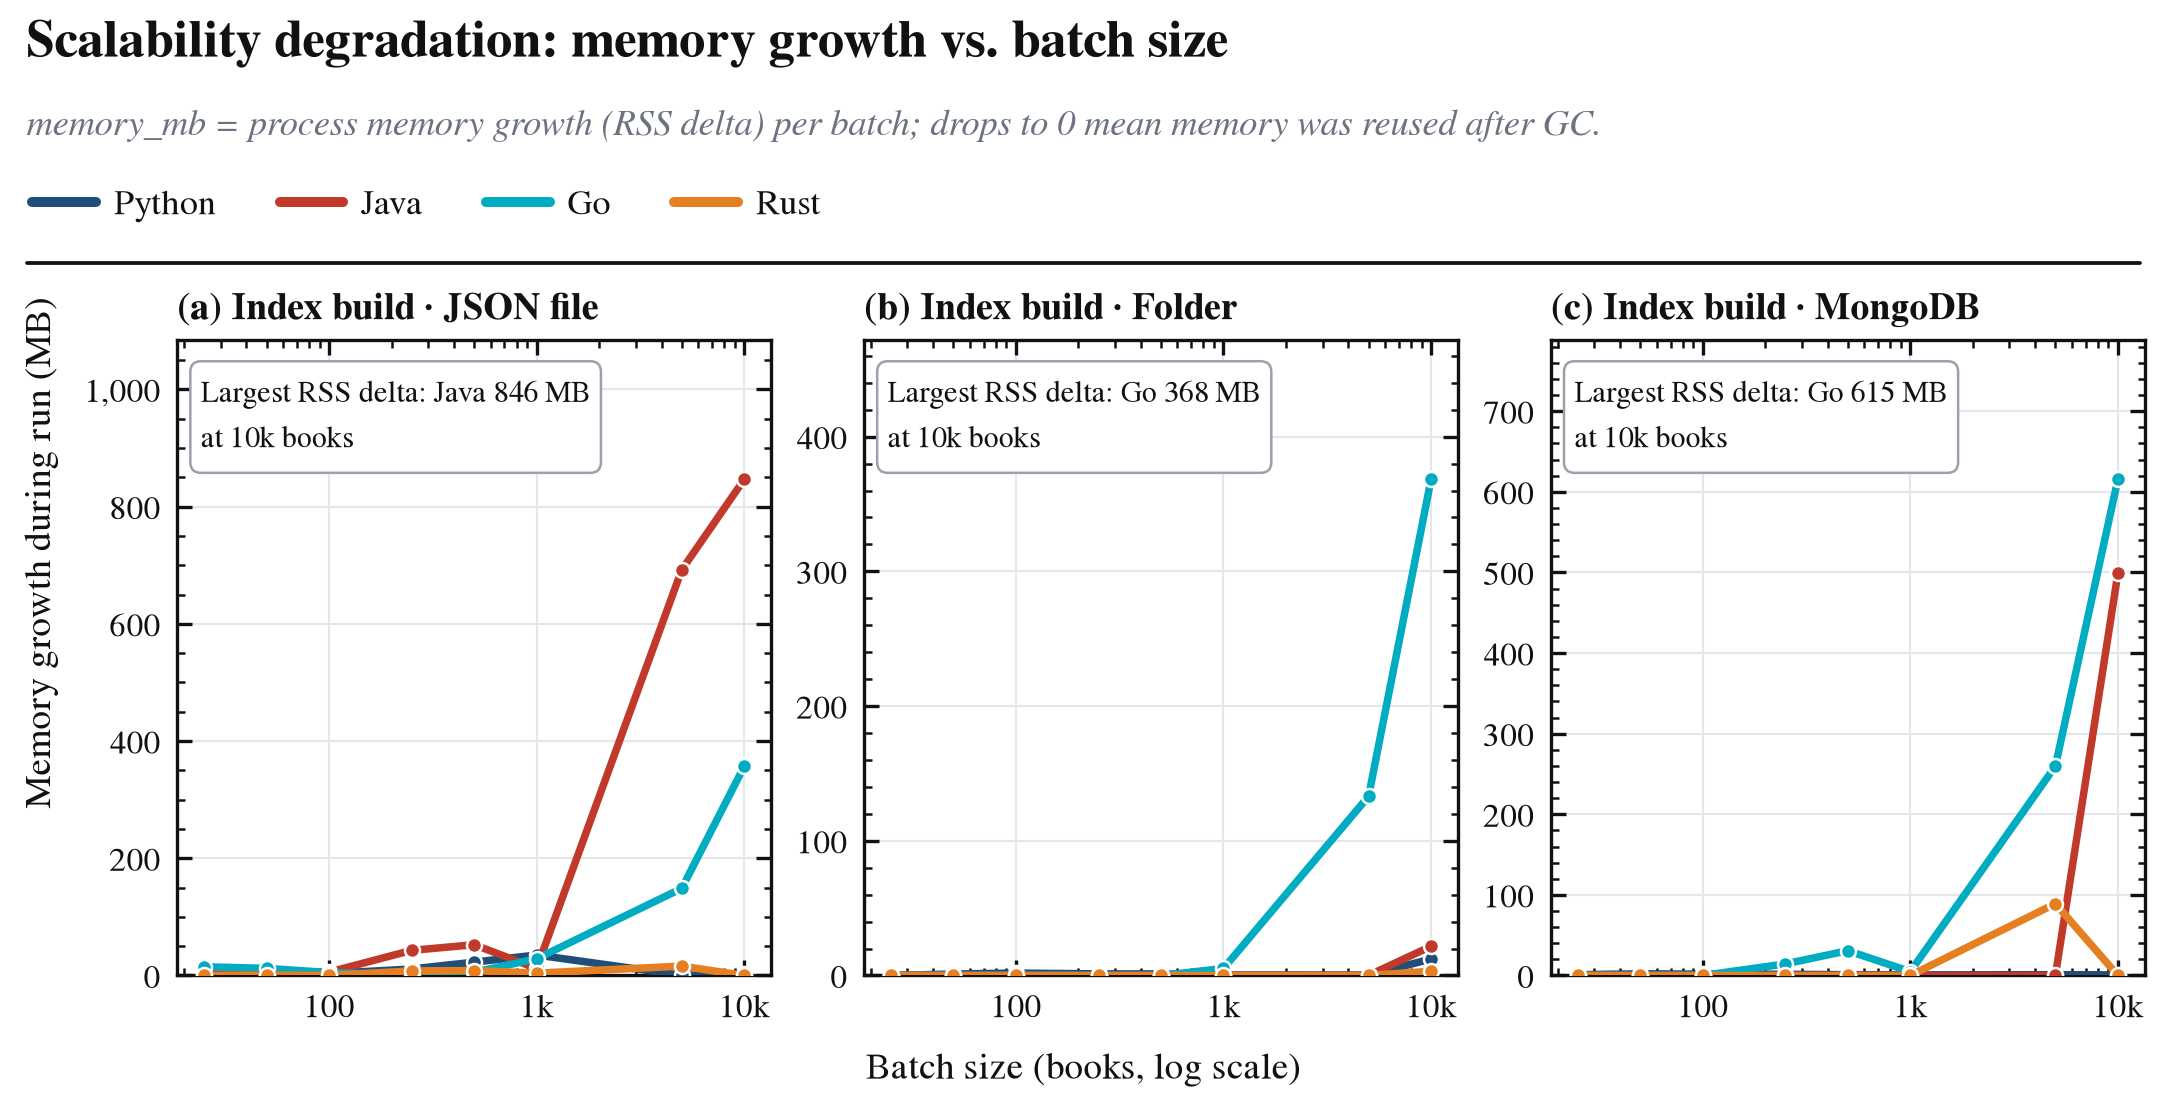
\includegraphics[width=0.94\textwidth]{scalability/scalability_memory.png}
        \caption{Memory growth versus batch size: \textbf{memory\_mb is the
        RSS delta per batch} in MiB, negative deltas reported as 0
        (\cref{tab:metrics}); the callout ``Largest RSS delta'' is the
        largest plotted delta, \emph{not} a process peak
        (\texttt{peak\_rss\_mb}). The subtitle's ``reused after GC'' is one
        possible reason for a zero, not a measured one.}
        \label{fig:scalability-memory}
    \end{minipage}
\end{figure}

\paragraph{Where the build time goes.}
At 10{,}000 books Go built every structure fastest (JSON 71.4~s, folder
78.4~s, MongoDB 83.8~s), followed by Python (170.9--215.3~s) and Rust
(198.1--208.1~s); Java took 1{,}130--1{,}185~s, 14--16$\times$ Go. Two
observations locate the bottleneck. First, within each implementation the
three structures cost nearly the same at 10{,}000 books (within 5\% in Rust
and Java, 17\% in Go, 26\% in Python) although they write very different
artefacts: at this size the build is dominated by the in-memory postings
construction that all three structures share, not by the storage back end.
The back end dominates at small batches instead, where the folder index pays
a fixed cost of one file per term (Python: 10.3~s at 25 books against
0.47~s for the JSON file). Second, the growth rates differ. Between 1{,}000
and 10{,}000 books the log--log slope is 0.81--1.05 for Python and Go,
1.06--1.16 for Rust and 1.26--1.33 for Java, so Java's JSON build grows from
20~ms per book at 25 books to 115~ms per book at 10{,}000, while Go's stays
between 6.5 and 9.5~ms per book.

\paragraph{Why the ports differ: three postings builders.}
The equivalence gate (\cref{sec:equivalence}) guarantees identical postings,
not identical data structures, and the source code shows three strategies
for the same output. The Go port appends a book ID to a term's slice after
an $O(1)$ check of the last element and sorts each slice once at the end. The
Rust port performs a hash lookup and a binary search into the growing
postings vector for every token occurrence. The Java port inserts every token
occurrence into a \texttt{TreeSet<Integer>}, allocating a boxed integer and
a tree node per posting, and copies each set into an \texttt{ArrayList} at
the end; all three Java structures build through this one method, which is
why their times coincide. The isolated \texttt{build\_postings} step over the
100-book corpus follows the same order (Go 0.57~s, Rust 0.88~s, Java 3.07~s;
not recorded by the Python harness), and Java's allocation-heavy strategy is
consistent with its super-linear growth, with process peaks of
5{,}000--5{,}763~MiB under a 5~GiB heap limit, and with the instability of
its JMH \texttt{buildPostings} score (\cref{sec:jmh}). That the data
structure rather than the language causes the gap is a hypothesis supported
by the code and the measurements, not one isolated by a controlled
experiment; it identifies the first optimisation target for Stage~2
(\cref{sec:future}).

\paragraph{The 1{,}601 MB figure.}
In an earlier version of this report a batch was said to ``require 1{,}601
MB''. That number was an RSS \emph{delta}, not a memory requirement and not
a process peak. In the current snapshot the largest plotted build delta is
846.5~MiB (Java, JSON file, 10{,}000 books). The largest delta anywhere in
the snapshot is 1{,}463.8~MiB, recorded by Go for one single-book update of
the 10{,}000-book JSON index (\texttt{benchmarks.csv}), an operation that
loads the whole index, merges one book and rewrites the file. Go's runtime
statistics for that operation show a heap growth of 1{,}267.7~MiB and
3{,}504~MiB allocated in total (\texttt{memstats.csv}), so the delta reflects
real allocation by the update. All four harnesses clamp negative deltas to
zero: a delta of 0 means the resident set did not grow, not that the
operation allocated nothing.

\paragraph{Peak RSS is a high-water mark.}
\texttt{peak\_rss\_mb} is the largest resident set observed while an
operation ran, sampled every \fixed{50}~ms, in a process that has already run
every earlier phase. Runtimes and allocators rarely return memory to the
operating system, so the series behaves as a high-water mark: Rust's peak
stays at 1{,}035.9--1{,}042.3~MiB across all eight folder builds, and Python
reports 3{,}411--3{,}616~MiB peaks for single-book updates of 25- to
1{,}000-book indexes, memory retained from the 10{,}000-book builds that ran
before them. A peak therefore cannot be attributed to the operation in its
row, and the earlier reading ``a peak well above its delta is the spike'' is
withdrawn. As a capacity observation only: the highest peaks were
7{,}304~MiB (Python, folder build of 10{,}000 books), 5{,}763~MiB (Java),
4{,}805~MiB (Go) and 2{,}981~MiB (Rust), on a virtual machine with
9{,}945~MiB of visible memory that also hosted \texttt{mongod}; Python's
peak is 73\% of it.

\paragraph{RAM spikes and garbage collection.}
The only direct collector evidence is Go's runtime record
(\texttt{memstats.csv}). Tokenising the 100-book corpus allocated 616~MiB
over 10 collections, and the 10{,}000-book JSON update allocated
3{,}504~MiB over 2 collections while its in-use heap reached 3{,}837~MiB;
with a single scheduler thread (\texttt{GOMAXPROCS=1}) these collections run
on the measured core. No GC log exists for Java, and recording one with
\texttt{-Xlog:gc} is the cheapest test of the collector hypothesis of
\cref{sec:refactor-effect}.

\subsection{Structures compared}
\label{sec:index-structures}

\paragraph{Where the bytes go.}
The repository also carries an interactive sankey diagram of the storage
breakdown (\texttt{charts/sankey/storage\_sankey.html}, generated by
\texttt{storage\_sankey.py} from \texttt{disk\_usage.csv}) that traces the
corpus bytes from datalake files into each index component; the static
figures of this report quote the same numbers
(\cref{tab:datalake-storage,tab:index-footprint}).

\paragraph{Query latency.}
Every structure answers the \fixed{30} shared queries, \fixed{5} times each
(\fixed{150} samples), on the index left by the 10{,}000-book build. Loading
the JSON file into memory is timed separately (\texttt{load\_json\_index}:
3.7~s Rust, 8.8~s Go, 16.7~s Java; not recorded by the Python harness) and
excluded from the query time. The ordering is the same in all four
implementations (\cref{fig:latency}): the in-memory JSON index is fastest
(0.64--2.68~ms mean), the folder index, which opens one small file per term,
second (1.01--3.84~ms), and MongoDB, which pays a round trip to the server
per term, slowest (4.25--8.31~ms, 1.3--4.8$\times$ the folder index). The
MongoDB means of Python, Go and Rust lie within 4.25--4.97~ms, consistent
with a cost dominated by the server round trip rather than by the client
language. Java's MongoDB mean is inflated by a tail of slow samples
(standard deviation 28.6~ms, maximum 348~ms), which we attribute, as a
hypothesis, to the driver's background threads and the collector sharing the
single pinned core. For every structure and language the standard deviation
is close to the mean: the 30 queries differ widely in cost (a query with an
absent term answers in microseconds), so the mean summarises a mixed
workload, and per-query medians and 95th percentiles are needed before any
latency claim finer than this ordering.

\paragraph{On-disk footprint.}
\Cref{tab:index-footprint} reports the state after the update phase (a
1{,}000-book base plus five single-book additions), which is when the harness
measures it; the 100-book and 10{,}000-book states were not measured.

\begin{table}[htbp]
    \centering
    \caption{Index footprint after the update phase (\texttt{disk\_usage.csv};
    apparent sizes in MiB).}
    \label{tab:index-footprint}
    \begin{tabular}{@{}lccc@{}}
        \toprule
        Structure & Size (MiB) & Files & Directories \\
        \midrule
        JSON file & 75.92 & 1 & 0 \\
        Folder & 42.13 & 106{,}479 & 26 \\
        MongoDB (\texttt{collStats storageSize}) & 5.4--29.6 & --- & --- \\
        \bottomrule
    \end{tabular}
\end{table}

The JSON and folder figures are byte-identical in the four implementations,
as equivalence predicts. The folder figure is an apparent size: at a 4~KiB
block size its 106{,}479 files cannot occupy less than 415.9~MiB of allocated
space, so on a block-based filesystem the folder index is likely the most
expensive structure rather than the cheapest (allocation was not measured).
For MongoDB the client-side file scan is meaningless, so the server's
\texttt{collStats storageSize} is read instead; the collection is dropped and
re-created before every build, in every language. Even so, identical logical
content yields 5.4~MiB (Go), 13.1 (Java), 16.1 (Rust) and 29.6~MiB (Python).
One plausible cause is that \texttt{storageSize} reflects what the storage
engine has written by its last checkpoint, so it depends on when the
statistic is read; we have not verified this. The MongoDB size is therefore
reported, not compared, and no footprint conclusion rests on it.

\subsection{Incremental updates}
\label{sec:index-updates}

Construction cost and update cost are different questions, so updates are
measured separately (\cref{fig:updates}). A base index of \fixed{25, 50,
250, 500, 1000} books is built untimed; then five single-book additions with
fresh synthetic IDs, which cannot collide with the base, are timed one by
one, and their mean is plotted. Every added book carries the same tokens,
computed before timing starts, so tokenisation is not part of the update
time and each addition merges IDs into existing terms without creating new
ones.

\begin{figure}[htbp]
    \centering
    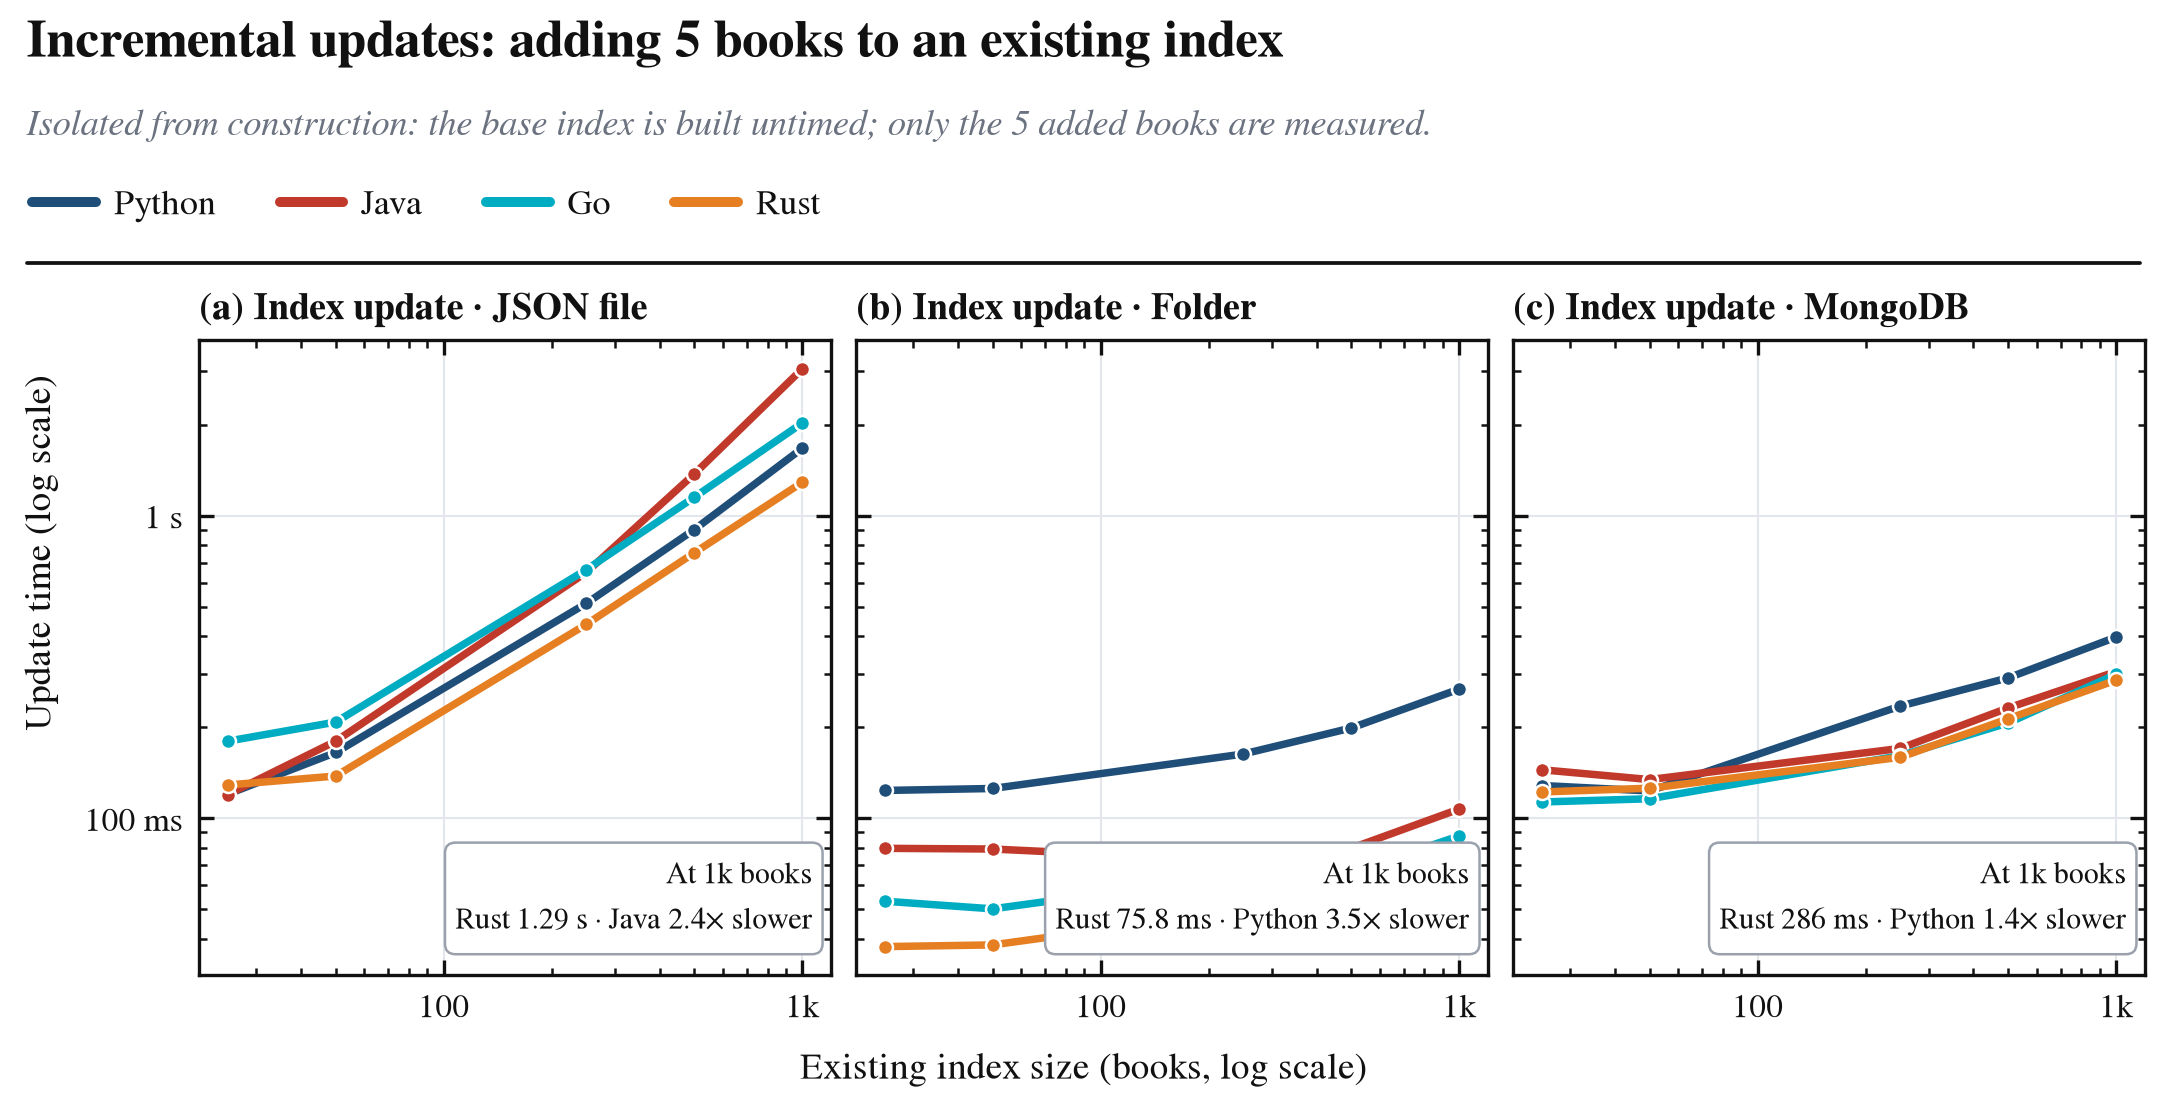
\includegraphics[width=0.72\textwidth]{scalability/scalability_updates.png}
    \caption{Incremental update time versus base index size, isolated from
    construction (\texttt{updates.csv}). Each point is the mean of five
    single-book additions; the ``5 books'' in the figure title are those
    five repetitions, not one five-book batch.}
    \label{fig:updates}
\end{figure}

\paragraph{The O(1) claim.}
The earlier report said MongoDB updates were ``O(1)''. The operation is
\texttt{update\_book}: one upsert per distinct term of the added book, sent
as a single unordered bulk write in all four ports since the current
snapshot. Each upsert runs an update pipeline (\texttt{\$setUnion} followed
by \texttt{\$sortArray}) that rebuilds and re-sorts that term's \emph{whole}
postings array, so the cost depends on the number of terms in the added book
\emph{and} on the postings length of those terms, which grows with the index.
The measurements agree. From base 25 to 1{,}000 the mean update time grew
10.0--25.5$\times$ for the JSON file, 1.35--2.16$\times$ for the folder index
and 2.11--3.09$\times$ for MongoDB. One further single-book update per
structure was timed on the 10{,}000-book index left by the build sweep
(\texttt{benchmarks.csv}, one sample each): JSON 13.1--28.6~s, folder
0.39--1.77~s, MongoDB 2.64--2.92~s. From base 1{,}000 to 10{,}000 the
MongoDB update grew 7.3--9.2$\times$ for a $10\times$ larger base, close to
linear, as expected when the corpus is repeated and a term's postings array
grows in proportion to the base. No structure showed constant update cost;
the O(1) claim is withdrawn and replaced by these curves, and no behaviour is
asserted beyond the measured range (\cref{sec:limitations}).

\paragraph{Which structure updates fastest.}
The folder index had the lowest update time in 18 of the 20
language--base-size points; both exceptions are Python at the smallest bases,
where the JSON file (base 25) and MongoDB (base 50) were 3\% and 2\% faster.
At base 1{,}000 it took 76--267~ms, against
286--397~ms for MongoDB and 1.29--3.06~s for the JSON file. Two
qualifications apply. First, durability is not equal across structures: the
JSON file is written through a temporary file, \texttt{fsync} and rename,
whereas every port rewrites the folder index's term files with plain,
unsynchronised writes, and no port requests more than MongoDB's default
write concern. Part of the folder index's advantage is therefore paid for
with weaker crash guarantees. Second, the MongoDB server runs in its own,
unpinned container, so its share of the work is not bounded by the client's
single-core budget; during the base-10{,}000 update the client itself used
0.4--6.8\% CPU, waiting on the server.

\subsection{Memory and disk of the MongoDB structure}
\label{sec:index-memory}

All client-side memory series (\texttt{memory\_mb}, \texttt{peak\_rss\_mb})
describe the benchmark process only, so \texttt{mongod}'s resident memory is
\emph{not} included in any client figure. The server's cost appears instead
as its own storage, measured through \texttt{collStats storageSize} on the
benchmark database (\texttt{search\_engine\_benchmark}), and as the extra
process a deployment must run. Any capacity statement about MongoDB in this
report refers to that measured size at the measured corpus, plus the
unmeasured server memory, which is listed as a limitation. The server's CPU
is not measured either, and its container has no CPU limit
(\texttt{docker-compose.yml}), so MongoDB-backed phases receive server-side
compute outside the single-core budget of the client
(\cref{sec:host}).
